\section{Experiments}
\label{sec:experiments}

\subsection{Datasets and Protocol}
\label{sec:protocol}

We evaluate on four public binary-segmentation datasets that span three modalities and very different target morphology: BUSI breast ultrasound~\cite{aldhabyani2020busi} (low-contrast lesions with diffuse borders), GlaS gland histology~\cite{sirinukunwattana2017glas} (many touching objects per image), and the CVC-ClinicDB~\cite{bernal2015cvc} and Kvasir-SEG~\cite{jha2020kvasir} colonoscopy collections (one or few polyps of variable size). All images are resized to $256\times256$ pixels (the public repository uses larger resolutions for some datasets; both models here share one resolution, so the comparison is internal to this protocol).

The protocol is that of the public U-KAN code~\cite{li2025ukan} and is frozen for every run in this article: an $80/20$ train/validation split drawn with data seed $2981$, $6142$ or $1187$; batch size $8$; Adam with learning rate $10^{-4}$ and weight decay $10^{-4}$ ($10^{-2}$ for the Kolmogorov--Arnold layers, as in the backbone, with $\theta$ and $\beta$ excluded from weight decay); cosine annealing to $10^{-5}$; $400$ epochs; binary cross-entropy plus Dice as the segmentation loss; and a fixed initialisation seed. For a given data seed the backbone and the routed model see exactly the same split and the same mini-batch order. No test-time augmentation, post-processing or morphological cleaning is applied. The public protocol defines no separate test partition, so all numbers are validation results and are labelled as such; model selection takes the epoch of highest validation intersection over union (IoU), and Dice is read at that epoch. Because the reported quantity is a maximum over epochs, we also report the mean over the last $50$ epochs, which is free of checkpoint selection; both rules are reported for every dataset throughout, and neither is chosen per dataset. All runs were executed with PyTorch~2.11 and CUDA~12.8 on a single NVIDIA GeForce RTX~5090D. On an idle GPU, batch-1 inference at $256\times256$ takes $12.0\pm0.05$\,ms for the backbone and $17.2\pm0.4$\,ms with ACRE-C (mean $\pm$ s.d.\ over the $33$ GlaS validation images), an increase of $5.2$\,ms ($43\%$); epoch times recorded during training were taken on a shared GPU and are not reported.

Beyond IoU and Dice we report, from the selected checkpoints, the $95$th-percentile Hausdorff distance (HD95), the average symmetric surface distance (ASSD) and the boundary F-score at a two-pixel tolerance (BF$_2$), all computed per image at $256\times256$ and averaged. Where the model changes the boundary rather than the interior, these are the metrics that should move.

\subsection{Evaluation Plan and Screening Gates}
\label{sec:gates}

The design and the screening conditions below were fixed before any run was started, so that the results can be judged against a bar set in advance rather than one chosen afterwards. (G) On split $2981$ the routed model must reach at least the validation IoU of a previous internal design with three ported modules: $85.5$, $87.0$, $78.5$ and $71.5$ on GlaS, CVC-ClinicDB, Kvasir-SEG and BUSI, and the GlaS component ladder must be monotone within $0.2$ points. (D) The polarity must not drift: the cell-level cross-entropy of $p$ may not rise by more than $0.02$, nor its cell IoU fall by more than one point, between epochs $50$--$100$ and the last $50$; the spatial standard deviation of $\rho$ must exceed $0.05$; and expert output-layer norms must stay below $10$. (U) On GlaS the learned abstention must beat the fixed policies \emph{margin} and \emph{none} by at least $0.2$ points. Runs that pass on split $2981$ are repeated on the two remaining seeds.

\subsection{Main Results}
\label{sec:main-results}

\begin{table*}[!t]
\caption{Validation Results Under the Frozen Protocol (\%, Mean$\pm$Standard Deviation Over Three Data Seeds). Left: Best-Validation-IoU Checkpoint. Right: Mean IoU Over the Last 50 Epochs, Without Checkpoint Selection.}
\label{tab:main}
\centering\footnotesize
\begin{threeparttable}
\setlength{\tabcolsep}{4.5pt}
\begin{tabular}{@{}lccc ccc ccc@{}}
\toprule
Dataset & \multicolumn{3}{c}{IoU (best)} & \multicolumn{3}{c}{Dice (at best IoU)} & \multicolumn{3}{c}{IoU (last 50 epochs)} \\
\cmidrule(lr){2-4}\cmidrule(lr){5-7}\cmidrule(lr){8-10}
 & U-KAN & + ACRE-C & $\Delta$ & U-KAN & + ACRE-C & $\Delta$ & U-KAN & + ACRE-C & $\Delta$ \\
\midrule
BUSI & 69.27$\,\pm\,$6.44 & 68.82$\,\pm\,$6.41 & $-0.45$ & 80.84$\,\pm\,$5.05 & 80.56$\,\pm\,$5.07 & $-0.28$ & 66.15$\,\pm\,$7.32 & 67.14$\,\pm\,$6.04 & $+0.99$ \\
GlaS & 85.43$\,\pm\,$1.11 & 86.13$\,\pm\,$1.07 & $+0.70$ & 92.06$\,\pm\,$0.67 & 92.48$\,\pm\,$0.61 & $+0.41$ & 84.35$\,\pm\,$1.23 & 84.97$\,\pm\,$1.04 & $+0.62$ \\
CVC-ClinicDB & 88.11$\,\pm\,$1.31 & 88.73$\,\pm\,$0.99 & $+0.63$ & 93.63$\,\pm\,$0.76 & 93.99$\,\pm\,$0.56 & $+0.36$ & 87.47$\,\pm\,$1.38 & 88.13$\,\pm\,$1.03 & $+0.66$ \\
Kvasir-SEG & 76.99$\,\pm\,$1.19 & 79.09$\,\pm\,$0.26 & $+2.10$ & 86.63$\,\pm\,$0.86 & 87.97$\,\pm\,$0.32 & $+1.34$ & 75.25$\,\pm\,$1.52 & 77.53$\,\pm\,$0.54 & $+2.28$ \\
\midrule
Mean $\Delta$ over datasets &  &  & $+0.75$ &  &  & $+0.46$ &  &  & $+1.14$ \\
\bottomrule
\end{tabular}
\begin{tablenotes}[flushleft]\footnotesize
\item All runs: $256\times256$, batch 8, Adam $10^{-4}$, cosine schedule, 400 epochs, identical split and mini-batch order for both models within a seed. Parameters: U-KAN 6.36\,M, + ACRE-C 6.75\,M. A superscript marks the number of seeds when fewer than three were available.
\end{tablenotes}
\end{threeparttable}
\end{table*}


Table~\ref{tab:main} compares U-KAN, re-trained under the frozen protocol, with U-KAN + ACRE-C over the three data seeds. The three-seed mean rises on GlaS ($+0.70$), CVC-ClinicDB ($+0.62$) and Kvasir-SEG ($+2.10$) and is level on BUSI ($-0.45$ at the best epoch, $+0.99$ on the last-$50$ mean), a four-dataset average of $+0.75$. The seed spread (sample s.d.) narrows on Kvasir-SEG ($1.19$ to $0.26$) and CVC-ClinicDB ($1.31$ to $0.99$) and is unchanged on GlaS ($1.11$ to $1.07$) and BUSI ($3.72$ to $3.70$). The paired per-seed differences are $0.70\pm0.73$ on GlaS, $0.63\pm0.43$ on CVC-ClinicDB, $2.10\pm0.98$ on Kvasir-SEG and $-0.45\pm0.86$ on BUSI (mean$\pm$s.d.); with three seeds these are paired observations, not significance tests. Gate~(G) failed on BUSI at split $2981$ ($69.02$ against $71.5$); the twelve-run protocol was completed regardless, because the gates are screening conditions fixed before training rather than acceptance criteria, and the failure is reported rather than absorbed. The per-seed values in Table~\ref{tab:perseed} show that the direction is consistent: eleven of the twelve seed-level comparisons are positive, the exception being BUSI seed $2981$ ($-1.64$); the GlaS and CVC seed-$1187$ values are the two smallest positive ones ($+0.03$ and $+0.06$). The added cost is $0.39$\,M parameters and $16\%$ of the multiply--accumulate operations (Section~\ref{sec:complexity}).

\begin{table}[!t]
\caption{Per-Seed Best Validation IoU (\%): U-KAN $\rightarrow$ U-KAN + ACRE-C}
\label{tab:perseed}
\centering\footnotesize
\begin{tabular}{@{}lccc@{}}
\toprule
Dataset & Seed 2981 & Seed 6142 & Seed 1187 \\
\midrule
BUSI & 70.66$\,\rightarrow\,$69.02 & 62.25$\,\rightarrow\,$62.31 & 74.90$\,\rightarrow\,$75.12 \\
GlaS & 84.66$\,\rightarrow\,$86.36 & 86.70$\,\rightarrow\,$87.07 & 84.93$\,\rightarrow\,$84.96 \\
CVC-ClinicDB & 86.59$\,\rightarrow\,$87.64 & 88.80$\,\rightarrow\,$89.57 & 88.92$\,\rightarrow\,$88.98 \\
Kvasir-SEG & 75.69$\,\rightarrow\,$79.15 & 78.03$\,\rightarrow\,$79.32 & 77.24$\,\rightarrow\,$78.81 \\
\bottomrule
\end{tabular}
\end{table}


\begin{table}[!t]
\caption{Boundary Metrics From the Best Checkpoints (Mean Over Seeds; HD95 and ASSD in Pixels at $256\times256$, BF$_2$ in \%)}
\label{tab:boundary}
\centering\footnotesize
\begin{tabular}{@{}llccc@{}}
\toprule
Dataset & Method & HD95 $\downarrow$ & ASSD $\downarrow$ & BF$_2$ $\uparrow$ \\
\midrule
BUSI & U-KAN & 25.04$\,\pm\,$7.66 & 9.89$\,\pm\,$3.20 & 54.89$\,\pm\,$4.17 \\
 & + ACRE-C & 25.98$\,\pm\,$6.50 & 9.15$\,\pm\,$2.39 & 54.83$\,\pm\,$3.58 \\
\addlinespace[2pt]
GlaS & U-KAN & 20.57$\,\pm\,$2.95 & 3.91$\,\pm\,$0.51 & 74.12$\,\pm\,$0.95 \\
 & + ACRE-C & 16.62$\,\pm\,$4.52 & 3.36$\,\pm\,$0.66 & 75.26$\,\pm\,$1.04 \\
\addlinespace[2pt]
CVC-ClinicDB & U-KAN & 11.95$\,\pm\,$2.20 & 3.08$\,\pm\,$0.33 & 74.66$\,\pm\,$1.46 \\
 & + ACRE-C & 11.83$\,\pm\,$0.48 & 3.71$\,\pm\,$0.33 & 76.97$\,\pm\,$2.25 \\
\addlinespace[2pt]
Kvasir-SEG & U-KAN & 26.41$\,\pm\,$1.94 & 7.50$\,\pm\,$0.66 & 65.36$\,\pm\,$0.19 \\
 & + ACRE-C & 23.79$\,\pm\,$1.36 & 6.63$\,\pm\,$0.40 & 68.10$\,\pm\,$0.96 \\
\bottomrule
\end{tabular}
\end{table}


Table~\ref{tab:boundary} reports the boundary metrics of the same checkpoints. The distance metrics move with IoU where IoU moves: HD95 falls by $3.95$ pixels on GlaS and $2.62$ on Kvasir-SEG, ASSD by $0.55$ and $0.87$, and BF$_2$ rises by $1.1$--$2.7$ points on the three datasets whose mean IoU improves. On CVC-ClinicDB BF$_2$ rises by $2.3$ while ASSD is the one distance metric that worsens ($3.08$ to $3.71$ pixels); on BUSI, where mean IoU does not improve, HD95 is unchanged within the seed spread ($25.04$ to $25.98$ against $\pm 7.7$) and ASSD falls slightly.

\subsection{Component Ladder and Ablations}
\label{sec:ablation}

\begin{table}[!t]
\caption{Component Ladder and Side Ablations on GlaS (Split 2981, 400 Epochs, Validation IoU/Dice at the Best Epoch and Mean IoU over the Last 50 Epochs, \%)}
\label{tab:ablation}
\centering\footnotesize
\setlength{\tabcolsep}{3.0pt}
\begin{tabular}{@{}lcccc@{}}
\toprule
Configuration & IoU & Dice & $\Delta$IoU & IoU$_{50}$ \\
\midrule
U-KAN (all switches off) & 84.53 & 91.51 & -1.83 & 83.62 \\
+ commit controller, $\mathcal{L}_{\mathrm{ctrl}}$ & 85.47 & 92.07 & -0.89 & 84.62 \\
+ consensus routers (local) & 86.01 & 92.38 & -0.35 & 85.03 \\
+ image-wide consensus, $\mathcal{L}_{\mathrm{foc}}$ (full) & 86.36 & 92.57 & +0.00 & 85.04 \\
\midrule
abstention fixed: \emph{margin} ($\rho\equiv1$) & 86.13 & 92.47 & -0.23 & 85.20 \\
abstention fixed: \emph{none} ($\rho\equiv0$) & 85.68 & 92.20 & -0.68 & 84.10 \\
full without detail trust (Step~1) & 85.87 & 92.31 & -0.49 & 84.80 \\
focus weight $z_{\mathrm{gt}}$ only (\emph{focus-gt}) & 86.52 & 92.65 & +0.16 & 85.82 \\
both losses, no routers (\emph{loss-only}) & 84.99 & 91.79 & -1.37 & 83.82 \\
\bottomrule
\end{tabular}
\end{table}


Table~\ref{tab:ablation} adds the components one at a time on GlaS (split $2981$, full $400$-epoch schedule for every row) and then removes or fixes individual parts of the complete model. The row with every switch off re-trains the backbone inside the v2 code path and lands within $0.13$ points of the separately trained U-KAN of Table~\ref{tab:main} ($84.53$ against $84.66$), so the ladder is read against a reproduced baseline. The ladder is monotone under both selection rules: the controller and its loss add $0.94$ points ($+1.00$ on the last-$50$ mean), the local consensus routers a further $0.54$ ($+0.41$), and the image-wide consensus with the focus loss a further $0.35$ ($+0.01$). The last step therefore shows at the best epoch but not on the last-$50$ mean, and we do not claim it beyond that.

Fixing the abstention to \emph{none}, which removes the third state altogether and reduces each router to a two-way consensus driven by the supervised polarity, costs $0.68$ points at the best epoch and $0.94$ on the last-$50$ mean; it also falls below the router-free row above it ($85.68$ against $86.01$), so two experts routed by a hard supervised map are worse than one plain residual. Fixing it to \emph{margin}---every cell withholds its whole margin, $\rho\equiv1$---costs $0.23$ points at the best epoch and gains $0.16$ on the last-$50$ mean, which is within the noise of one seed. The pre-specified gate~(U) is therefore met against \emph{none} and not decided against \emph{margin}: a soft third state is what makes the routing useful on this dataset, whereas learning where to withhold it, as against withholding the full margin everywhere, is not distinguishable here. Removing the bounded detail trust of Step~1 costs $0.49$ points at the best epoch and $0.24$ on the last-$50$ mean, and leaves the per-image boundary metrics essentially unchanged (HD95 $14.31$ against $13.72$ pixels, ASSD $2.98$ against $3.01$). Without it the model still gains $1.34$ points over the row with every switch off, so about three quarters of the total gain is carried by the controller, the consensus and the routed experts. Building the focus loss from the label band alone (\emph{focus-gt}), that is, dropping the detached abstention from the weight $\omega$ in (\ref{eq:lfoc}), does not hurt: IoU is $86.52$ at the best epoch ($+0.16$) and $85.82$ on the last-$50$ mean ($+0.78$), and the per-image boundary metrics improve (HD95 $11.78$ against $13.72$ pixels, ASSD $2.73$ against $3.01$, BF$_2$ $75.3$ against $74.1$). Reading the abstention back into the loss weighting therefore contributes nothing measurable on this dataset and seed, and the simpler weight $\omega=z_{\mathrm{gt}}$ is at least as good. We keep the pre-specified configuration as the reported model, since the twelve-run protocol of Table~\ref{tab:main} was fixed before this ablation was run, and flag $\omega=z_{\mathrm{gt}}$ as the recommended simplification. Finally, keeping both auxiliary losses but no routers (\emph{loss-only}) reaches $84.99$ at the best epoch and $83.82$ on the last-$50$ mean: $0.46$ and $0.20$ points above the row with every switch off, $1.37$ and $1.22$ below the full model, and below the controller-only row ($85.47$), which has $\mathcal{L}_{\mathrm{ctrl}}$ but not $\mathcal{L}_{\mathrm{foc}}$. The objective on its own therefore accounts for a small part of the gain, and the abstention-weighted focus loss without routers is mildly harmful, consistent with the \emph{focus-gt} row: the abstention earns its place in the routing, not in the loss. The architecture, not the objective, carries the result.

\subsection{Behaviour of the Controller}
\label{sec:dynamics}

\begin{table}[!t]
\caption{Controller Dynamics (Validation, Last-50-Epoch Means). $\Delta$BCE / $\Delta$IoU: Change of the Cell-Level Polarity BCE / IoU From Epochs 50--100 to the Last 50.}
\label{tab:dynamics}
\centering\scriptsize
\setlength{\tabcolsep}{3pt}
\begin{tabular}{@{}lcccccc@{}}
\toprule
Run & Cell IoU & $\Delta$BCE & $\Delta$IoU & $\bar{M}_a$ & std$(\rho)$ & max $\lVert W\rVert$ \\
\midrule
BUSI / full / 1187 & 56.1 & -0.046 & +15.64 & 0.07 & 0.122 & 2.94 \\
BUSI / full / 2981 & 52.6 & -0.049 & +15.38 & 0.07 & 0.116 & 2.97 \\
BUSI / full / 6142 & 52.2 & -0.046 & +15.62 & 0.07 & 0.125 & 3.13 \\
GlaS / abst\_margin / 2981 & 83.2 & -0.195 & +14.74 & 0.23 & 0.000 & 1.94 \\
GlaS / abst\_none / 2981 & 83.3 & -0.180 & +13.86 & 0.00 & 0.000 & 0.94 \\
GlaS / ctrl / 2981 & 83.9 & -0.221 & +16.84 & 0.11 & 0.000 & -- \\
GlaS / full / 1187 & 81.7 & -0.323 & +21.42 & 0.13 & 0.048 & 2.08 \\
GlaS / full / 2981 & 83.2 & -0.232 & +17.02 & 0.16 & 0.068 & 2.00 \\
GlaS / full / 6142 & 84.0 & -0.312 & +20.61 & 0.13 & 0.060 & 2.06 \\
CVC / full / 1187 & 76.0 & -0.069 & +28.55 & 0.03 & 0.088 & 2.66 \\
CVC / full / 2981 & 77.7 & -0.059 & +28.77 & 0.03 & 0.089 & 2.62 \\
CVC / full / 6142 & 75.7 & -0.081 & +29.01 & 0.04 & 0.087 & 2.76 \\
Kvasir / full / 1187 & 67.5 & -0.053 & +14.06 & 0.07 & 0.066 & 3.08 \\
Kvasir / full / 2981 & 65.6 & -0.055 & +12.70 & 0.08 & 0.078 & 3.21 \\
Kvasir / full / 6142 & 67.2 & -0.067 & +15.99 & 0.07 & 0.083 & 3.16 \\
\bottomrule
\end{tabular}
\end{table}


Section~\ref{sec:controller} argued that, with the masses detached from $p$, the polarity receives no direct routing gradient but may still drift through the shared trunk. Table~\ref{tab:dynamics} reports the monitors that test this on every run with a controller. On every full-model run the cell-level cross-entropy of $p$ falls between epochs $50$--$100$ and the last $50$ epochs --- by $0.05$ on the polyp and ultrasound sets and by up to $0.32$ on GlaS --- and the cell IoU rises by $13$ to $29$ points, so the drift gates are met with margin on all twelve runs. The abstention settles at a mean mass $\bar M_a$ of $0.03$ to $0.17$, lowest on CVC-ClinicDB and highest on GlaS, with a spatial standard deviation of $\rho$ of $0.048$ to $0.125$: at or above the $0.05$ screening level on eleven of the twelve runs, with GlaS seed $1187$ at $0.048$ marginally below it. The controller therefore neither abstains everywhere nor collapses to a two-state field; the expert output-layer norms stay below $3.3$, far from the bound at which the residual could dominate the base evidence. The three runs whose abstention is not learned --- the router-free \emph{ctrl} row and the fixed \emph{margin} and \emph{none} policies --- hold std$(\rho)\equiv0.000$, the empirical signature of the claim in Section~\ref{sec:controller} that $\rho$ receives gradient only through the routers.

\subsection{Qualitative Results}
\label{sec:qualitative}

\begin{figure*}[!t]
\centering
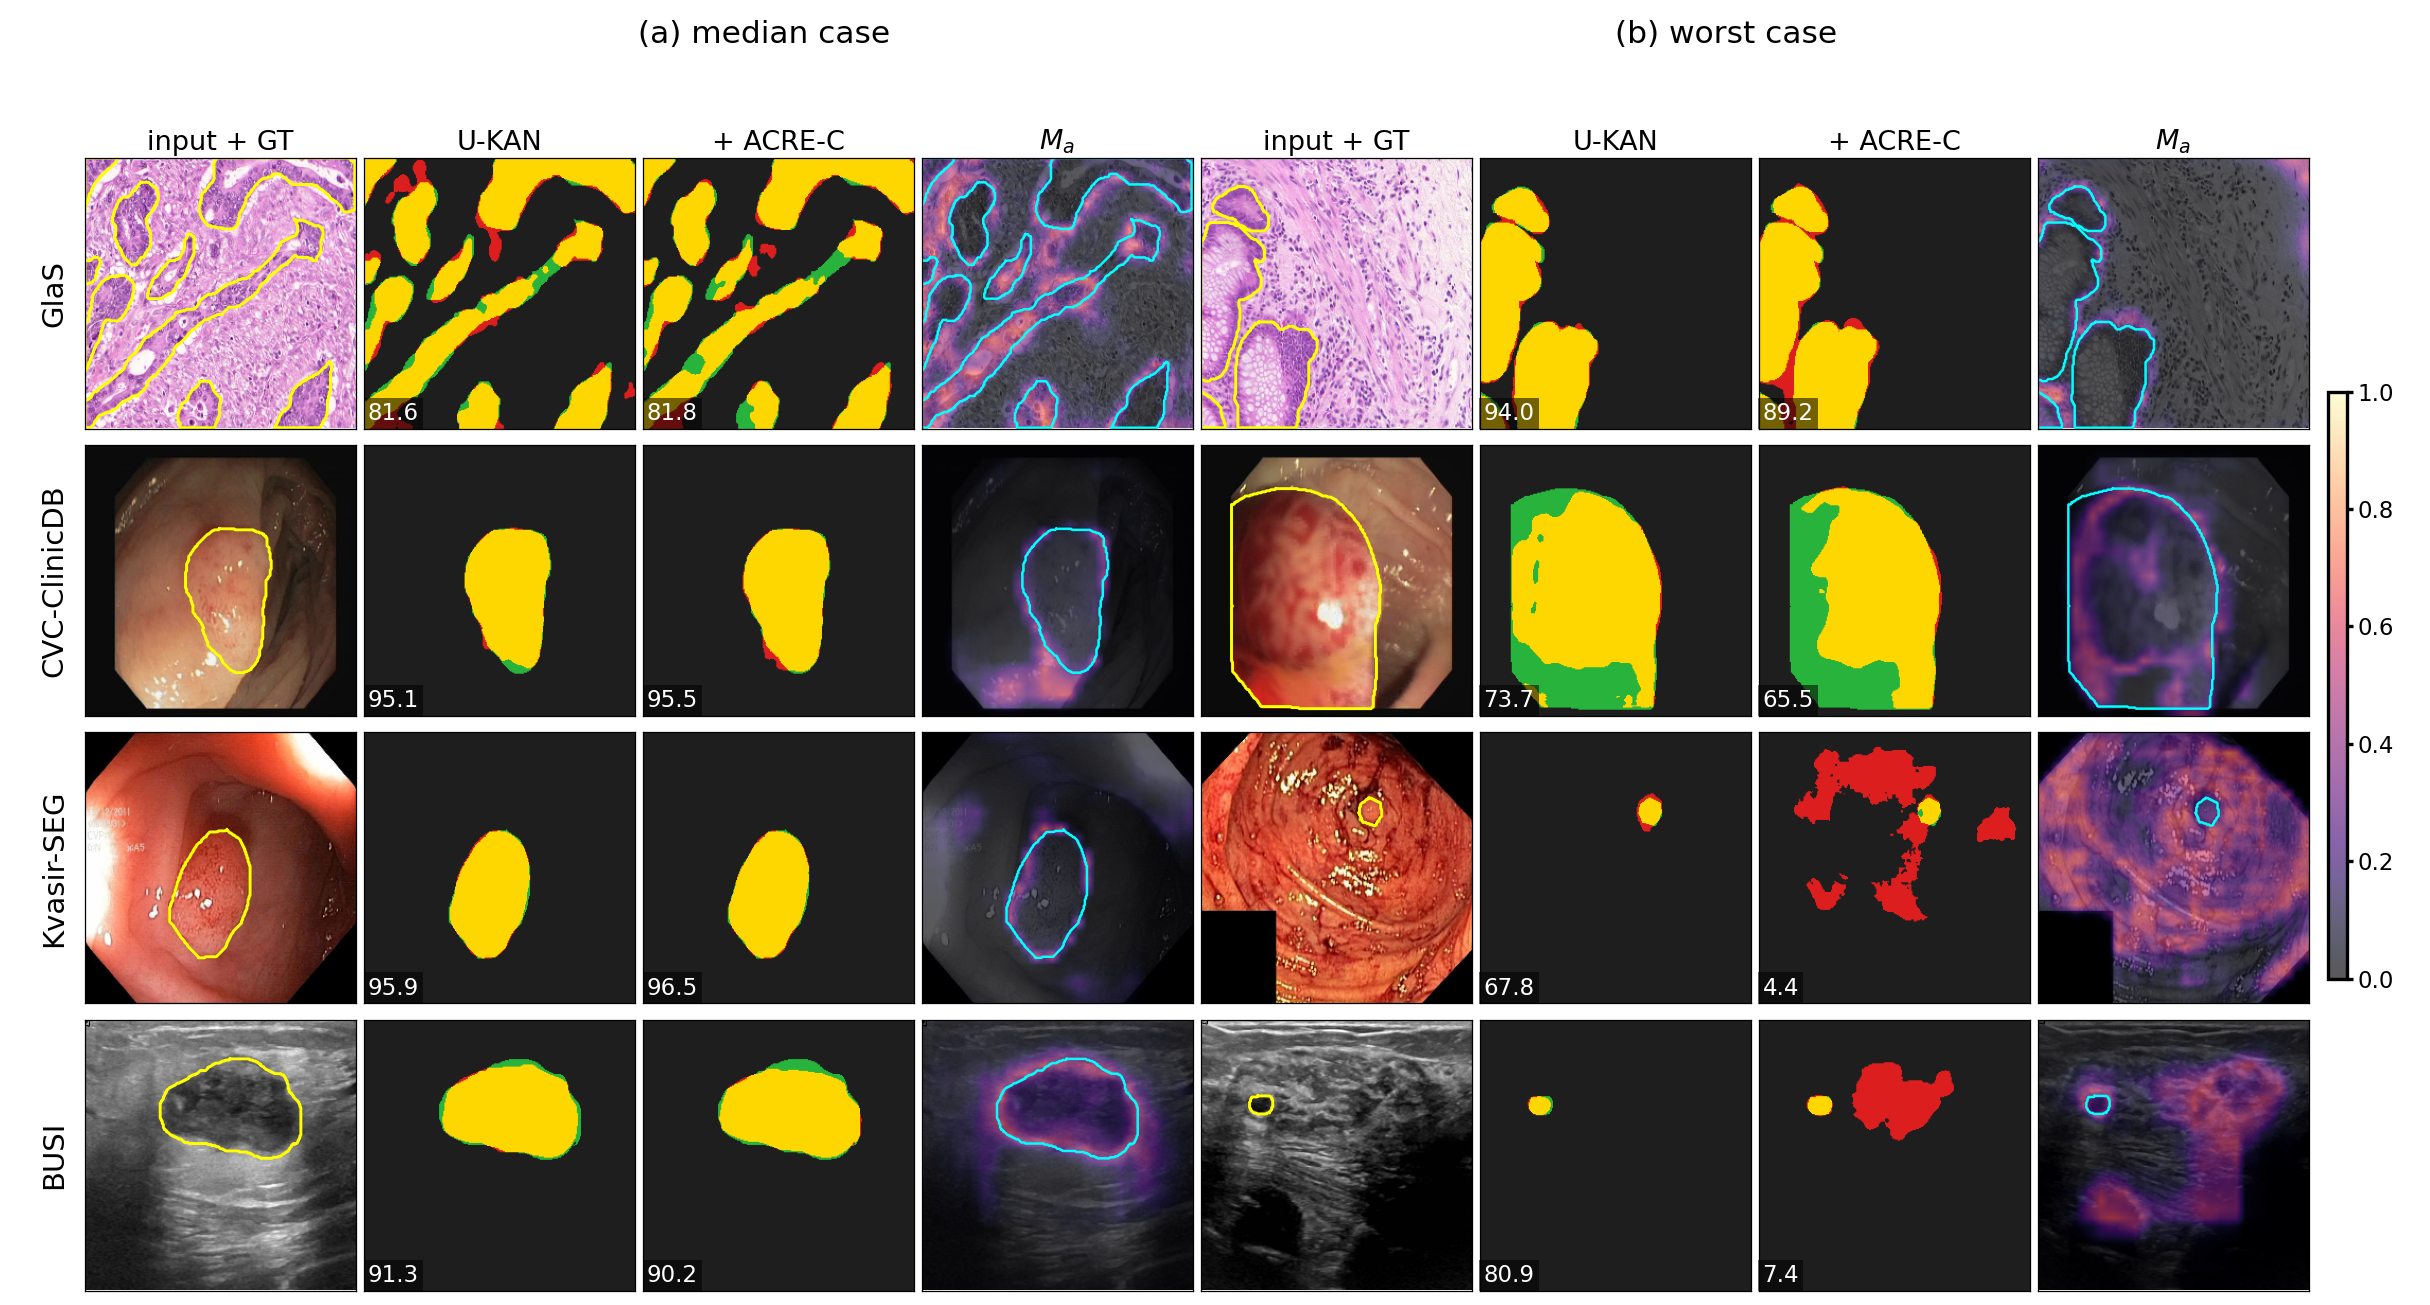
\includegraphics[width=0.75\textwidth]{figures/fig11_qual_grid.png}
\caption{Validation cases of split $2981$, one row per dataset: (a) the image at the median of the per-image IoU difference between the two models, (b) the image with the largest loss against U-KAN. Per block: input with ground-truth contour; error maps of U-KAN and of U-KAN\,+\,ACRE-C (yellow true positive, red false positive, green false negative, per-image IoU inset); the abstention mass $M_a$ ($H/8$ grid, bilinearly resampled) with the ground-truth contour in cyan. Failure cases are shown deliberately.}
\label{fig:qual}
\end{figure*}

Fig.~\ref{fig:qual} shows, for each dataset, the median validation case and the case with the largest loss against the backbone. Two regularities appear in the abstention maps. First, $M_a$ attaches to boundaries: on GlaS it follows the gland contours and the stroma between adjacent glands, on the polyp datasets it forms a rim around the lesion, and on the ultrasound it covers the lesion border and the acoustic shadow beneath it. It is near zero on unambiguous tissue. This is the pattern one expects of a mass that is withheld where the polarity's margin is small, and it was not supervised. Second, the failure cases share one mechanism. On Kvasir-SEG and BUSI the worst cases are a small target inside a large textured field (bleeding mucosa, heterogeneous breast tissue), the polarity abstains over much of that field ($M_a\approx0.3$--$0.5$), and the abstain expert adds false-positive regions there; the backbone, which does not route, does not make them. The worst GlaS and CVC-ClinicDB cases are of a different kind: a contour pushed outward at low $M_a$, and a frame-filling polyp whose left third is missed by both models with $M_a\approx0.3$ over the missed part. The abstention therefore marks where the model is undecided, but the routed expert can also act wrongly there, and the per-image tails of Table~\ref{tab:boundary} on BUSI come from this.
